\documentclass[border = 3pt]{standalone}

\usepackage{main}
\usepackage{tikz}

\begin{document}

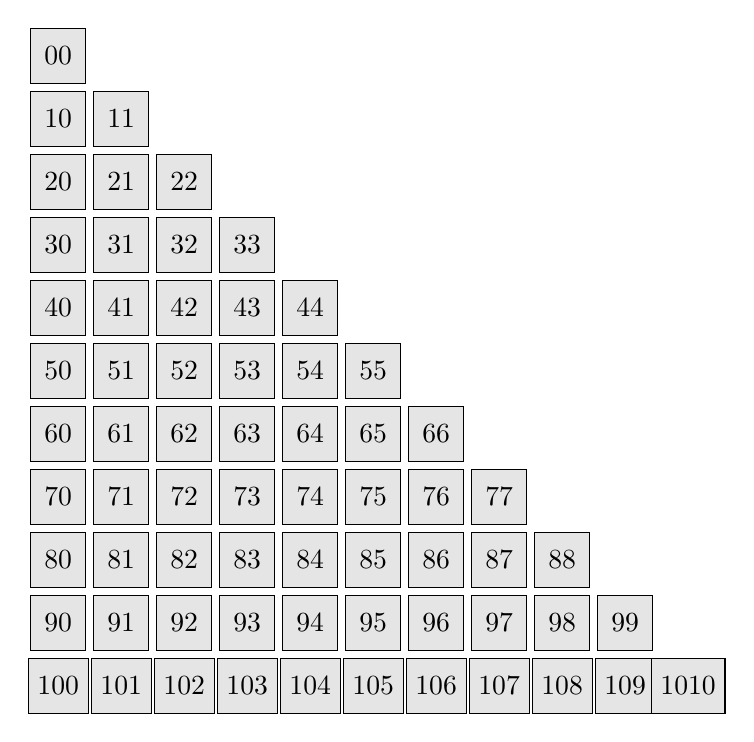
\begin{tikzpicture}[
  scale = 0.8,
  cnp/.style = {
    rectangle, draw,
    minimum size = 2em,
    fill         = gray!20,
  }
]
  \foreach \n in {0,...,10} {
    \foreach \p in {0,...,\n} {
      \draw (\p, 6 - \n) node[cnp] { \Cnp{\n}{\p} };
    }
  }
\end{tikzpicture}

\end{document}
